% Created 2024-08-31 Sat 10:06
% Intended LaTeX compiler: pdflatex
\documentclass[letterpaper, 12pt]{article}
\usepackage[utf8]{inputenc}
\usepackage[T1]{fontenc}
\usepackage{graphicx}
\usepackage{longtable}
\usepackage{wrapfig}
\usepackage{rotating}
\usepackage[normalem]{ulem}
\usepackage{amsmath}
\usepackage{amssymb}
\usepackage{capt-of}
\usepackage{hyperref}
\usepackage{minted}
\usepackage{xcolor}
\usepackage{hyperref}
\usepackage{tocloft}
\usepackage{minted}
\usemintedstyle{manni}
\usepackage{pdfpages}
\usepackage{fancyhdr}
\usepackage{graphicx}
\usepackage[top=1.4in, left=0.5in, right=0.5in, bottom=0.8in]{geometry}
\usepackage[T1]{fontenc}
\usepackage{helvet}
\pagestyle{fancy}
\renewcommand{\headrulewidth}{0pt}
\renewcommand{\footrulewidth}{0pt}
\setlength{\parindent}{0em}
\setlength{\parskip}{1em}
\usepackage{hyperref}
\usepackage {color}
\usepackage {tabularray}
\usepackage{xcolor}
\hypersetup{
colorlinks=true,
linkcolor=blue,
filecolor=magenta,
urlcolor=cyan,
citecolor=green,
pdfborder={0 0 0}
}
\usepackage[most]{tcolorbox}
\author{Hilduara Abreu}
\date{\today}
\title{PS192 | Protocolo de Estudiante Desaparecido\\\medskip
\large Versión en Español}
\hypersetup{
 pdfauthor={Hilduara Abreu},
 pdftitle={PS192 | Protocolo de Estudiante Desaparecido},
 pdfkeywords={},
 pdfsubject={},
 pdfcreator={Emacs 29.4 (Org mode 9.6.15)}, 
 pdflang={English}}
\begin{document}

\fancyfoot[C]{\setlength{\unitlength}{1in}\begin{picture}(5,0)\put(-1.8,-0.5){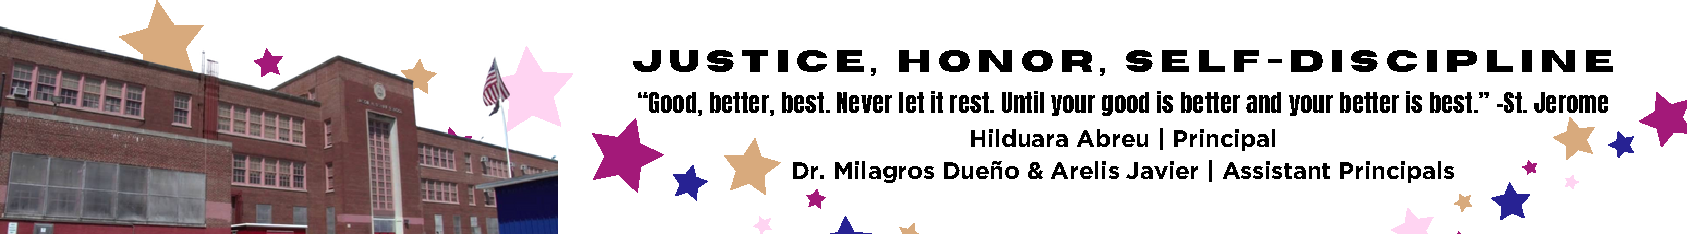
\includegraphics[width=8.8in,height=1.3in]{logo-1}}\end{picture}}
\fancyhead[C]{\setlength{\unitlength}{1in}\begin{picture}(5,0)\put(-1.9,-0.5){
\includegraphics[width=8.9in,height=1.3in]{logo-2}}\end{picture}}
\fancyhead[R]{\thepage}
\pagenumbering{gobble}

\begin{document}
\newpage
\vspace*{-0.3cm}

\textbf{Re: Implementación del Protocolo de Estudiantes Desaparecidos, efectivo a partir del 5 de septiembre de 2024}

Este Protocolo de Estudiantes Desaparecidos se establece para garantizar la seguridad y el bienestar de todos los estudiantes en PS192. Describe los pasos a seguir inmediatamente si se identifica que un estudiante está desaparecido, asegurando una respuesta rápida y eficiente por parte de todos los miembros del personal. El protocolo se alinea con las directrices del NYCDOE y el UFT y está diseñado para proporcionar claridad y coherencia en el manejo de situaciones críticas.

\textbf{Reportando a un Estudiante Desaparecido}
\begin{itemize}
\item \textbf{\textbf{Reporte Inmediato}}: Si un miembro del personal identifica a un estudiante desaparecido o nota que un estudiante elude la supervisión de un adulto, debe usar inmediatamente su teléfono celular para enviar un mensaje de texto a la administración y al coordinador de padres mientras busca o sigue al niño.
\item \textbf{\textbf{Activación del Equipo de Respuesta del Edificio (BRT)}}: Si se confirma que el estudiante está desaparecido, el Director activará el Equipo de Respuesta del Edificio (BRT) para ayudar a localizar al estudiante y prevenir que abandone las instalaciones.
\end{itemize}

\textbf{Esfuerzos de Búsqueda}
\begin{itemize}
\item \textbf{\textbf{Búsqueda Integral}}: El BRT y todo el personal disponible de la escuela realizarán una búsqueda exhaustiva tanto en áreas internas como externas en todo el recinto escolar.
\item \textbf{\textbf{Anuncio por Intercomunicador}}: Se hará un anuncio a través del intercomunicador de la escuela por parte de la secretaria, utilizando la frase en clave: "El león está fuera de la guarida. Llámame si lo ves o lo encuentras." Esta alerta notifica al personal sobre el estudiante desaparecido y ayuda a recopilar información sobre la última ubicación conocida del estudiante.
\item \textbf{\textbf{Notificación a las Autoridades}}: Si el estudiante no es encontrado en un tiempo específico, se notificará a la policía local. El Director y/o el presidente del BRT serán responsables de contactar al 911 e informar al Director de Seguridad del Distrito y al Superintendente del Distrito 6.
\item \textbf{\textbf{Perfil de Información del Estudiante}}: Una vez que lleguen las autoridades, el Director y/o el presidente del BRT proporcionarán un perfil de información del estudiante.
\end{itemize}

\textbf{Comunicación, Documentación y Retroalimentación}
\begin{itemize}
\item \textbf{\textbf{Notificación a los Padres/Tutores}}: La administración se pondrá en contacto con los padres o \newpage \vspace*{-0.5cm} tutores para informarles de la situación.
\item \textbf{\textbf{Documentación del Incidente}}: Los miembros del personal responsables de la supervisión del estudiante deben completar un formulario de informe OORS detallando el incidente antes de abandonar las instalaciones si el incidente ocurrió antes de la 1 p.m. El formulario será enviado a la Subdirectora, Dra. Milagros Dueño.
\item \textbf{\textbf{Revisión del Incidente}}: El Director revisará el formulario del incidente con el Líder del Capítulo del UFT y el presidente del BRT, recopilará comentarios y sugerencias, y puede convocar una reunión con los miembros del personal involucrados para una revisión y discusión adicionales.
\end{itemize}

\textbf{Medidas Preventivas}
\begin{itemize}
\item \textbf{\textbf{Monitoreo de Pasillos y Baños}}:
\begin{itemize}
\item \textbf{Segundo Piso}: Sra. Del Orbe, Sra. Cuesta, Sr. Abreu, y Sr. Suero supervisan el monitoreo del pasillo y los baños del segundo piso.
\item \textbf{Primer Piso}: Sra. Clemons, Sra. Rijo, y el designado por el director de MS 209 supervisan el pasillo y las instalaciones de baños del primer piso.
\end{itemize}
\item \textbf{\textbf{Seguridad en las Salidas}}: Sra. Clemons, nuestra agente de seguridad, inspeccionará y asegurará consistentemente todas las salidas para prevenir accesos no autorizados.
\item \textbf{\textbf{Educación en Seguridad para Estudiantes}}: Durante el bloque de SEL (Aprendizaje Socioemocional), los maestros proporcionarán a los estudiantes educación sobre procedimientos de seguridad y orientación sobre a quién contactar si se sienten perdidos o inseguros. Esto ocurrirá una vez al mes.
\end{itemize}

Su cooperación y estricta adherencia a este protocolo y las medidas preventivas descritas son cruciales para garantizar la seguridad y protección de nuestros estudiantes. Trabajando juntos y manteniendo la vigilancia, podemos contribuir significativamente a la seguridad general de nuestro entorno escolar.

Gracias por su atención y compromiso con la seguridad de nuestros estudiantes.

Con Justicia, Honor y Autodisciplina,


\includegraphics[width=0.16\textwidth]{hil_signature}

\textbf{Hilduara Abreu, Directora}

\href{www.ps192.org}{¡La escuela del Aprendizaje Alegre!}
\end{document}
